  \documentclass[xcolor=x11names,compress, 24pt]{beamer}
 %\documentclass[handout, t,xcolor=x11names,compress]{beamer}
 %% General document %%%%%%%%%%%%%%%%%%%%%%%%%%%%%%%%%%
 \usepackage{graphicx}
 \usepackage{tikz}
 \usetikzlibrary{arrows,shapes,snakes,automata,backgrounds}
 \usetikzlibrary{decorations.fractals}
 \usetikzlibrary{calc,through,backgrounds}
 \usepackage{graphics}
 \usepackage{setspace} 
 \usepackage{array, multirow}
 \usepackage{latexsym}
 \usepackage{qtree}
 \usepackage{beamerthemesplit}
 \usepackage{algorithmic}
 \usepackage{wrapfig}
 \usepackage{sidecap}
 \usepackage{apalike}
 %%%%%%%%%%%%%%%%%%%%%%%%%%%%%%%%%%%%%%%%%%%%%%%%%%%%%%
 
 \setbeamercolor{math text}{fg=blue!80!black}
 \setbeamercolor{normal text}{fg=blue!80!blue}
 
 \usepackage{supertabular,tabularx}
 \usepackage{listings}
 \usepackage{verbatim}
 \usepackage{color}
 \usepackage{setspace}
 %\usepackage{drop}
 
 
 
 
 %% Beamer Layout %%%%%%%%%%%%%%%%%%%%%%%%%%%%%%%%%%
 %\useoutertheme[subsection=false,shadow]{miniframes}
 %\useinnertheme{default}
 % \usecolortheme{seahorse}
 
 \usetheme{AnnArbor}
 %\useinnertheme[subsection=false,shadow]{rounded}
 %\useoutertheme{infolines}
 \usecolortheme{seahorse}
 \usefonttheme{serif,professionalfonts}
 %\usefonttheme{platino}

 
 \setbeamercolor{header}{fg=white,bg=DeepSkyBlue4}
 \setbeamercolor{frametitle}{bg=white,fg=DeepSkyBlue4}%, fontface=bf}
 \setbeamercolor*{section}{fg=white,bg=DeepSkyBlue4}%, fontface=bf}
 \setbeamercolor{title}{fg=white,bg=DeepSkyBlue4}
 \setbeamercolor{item}{fg=DeepSkyBlue4}
 \setbeamercolor*{lower separation line head}{bg=DeepSkyBlue4} 
 \setbeamercolor*{normal text}{fg=black,bg=white} 
 \setbeamercolor*{alerted text}{fg=red} 
 \setbeamercolor*{example text}{fg=black} 
 \setbeamercolor*{structure}{fg=black} 
 \setbeamercolor*{math text}{fg=blue!80!black}
 \setbeamercolor*{palette tertiary}{fg=black,bg=black!10} 
 \setbeamercolor*{palette quaternary}{fg=black,bg=black!10} 
 
  \newcommand{\rd}[1]{ \textcolor{red}{\textbf{#1}}}
 \newcommand{\bl}[1]{ \textcolor{DeepSkyBlue4}{\textbf{#1}}} 
 
 
 \setbeamerfont{title like}{shape=\scshape, series=\bfseries}
 \setbeamerfont{frametitle}{shape=\scshape, series=\bfseries}
 \setbeamerfont{normal text}{shape=\itshape, series=\bfseries}
 \setbeamerfont{item}{series=\bfseries}
 
 \definecolor{darkblue}{rgb}{0,0,0.6}
 \setbeamercolor{myfootline1}{fg=white,bg=DeepSkyBlue4}
 \setbeamercolor{myfootline2}{fg=white,bg=DeepSkyBlue4}
 
 \setbeamertemplate{headline}{
 	\leavevmode%
 	\hbox{\begin{beamercolorbox}[wd=.5\paperwidth,ht=2.5ex,dp=1.125ex,leftskip=.3cm,rightskip=.3cm]{myfootline1}%
 			\usebeamerfont{author in head/foot}	\insertsection
 		\end{beamercolorbox}%
 		
 		\begin{beamercolorbox}[wd=.5\paperwidth,ht=2.5ex,dp=1.125ex,leftskip=.3cm,rightskip=.3cm plus1fil]{myfootline2}%
 			\usebeamerfont{author in head/foot}\insertsubsection
 	\end{beamercolorbox}}%
 	\vskip0pt%
 }
 
 \setbeamertemplate{footline}{
 	\leavevmode%
 	\hbox{\begin{beamercolorbox}[wd=.5\paperwidth,ht=2.5ex,dp=1.125ex,leftskip=.3cm,rightskip=.3cm]{myfootline1}%
 			\usebeamerfont{author in head/foot}\insertshortauthor~~\insertshortinstitute
 		\end{beamercolorbox}%
 		
 		\begin{beamercolorbox}[wd=.5\paperwidth,ht=2.5ex,dp=1.125ex,leftskip=.3cm,rightskip=.3cm plus1fil]{myfootline2}%
 			\usebeamerfont{title in head/foot}\insertshorttitle\hfill\insertpagenumber
 	\end{beamercolorbox}}%
 	\vskip0pt%
 	\addtocounter{framenumber}{-1}
 }
 %\setbeamerfont{frametitle}{shape=\scshape,series=\bfseries,size={\fontsize{18}{36}}}
 
 
 \renewcommand{\(}{\begin{columns}}
 \renewcommand{\)}{\end{columns}}
\newcommand{\<}[1]{\begin{column}{#1}}
\renewcommand{\>}{\end{column}}


\usepackage{xpatch}
\setlength{\columnsep}{1cm}


\xpatchcmd{\itemize}
{\def\makelabel}
{\usebeamertemplate{itemize body}\def\makelabel}
{}{}


\xpatchcmd{\description}
{\def\makelabel}
{\usebeamertemplate{description body}\def\makelabel}
{}{}


\xpatchcmd{enumerate}
{\def\makelabel}
{\usebeamertemplate{enumerate body}\def\makelabel}
{}{}
\defbeamertemplate*{itemize body}{default}{
\setlength{\itemsep}{2cm}%
} % default is doing nothing

\setbeamertemplate{itemize body}{%
\setlength{\itemsep}{0.2cm}%
}

\setbeamertemplate{description body}{%
\setlength{\itemsep}{0.2cm}%
}

\setbeamertemplate{enumerate body}{%
\setlength{\itemsep}{0.2cm}%
}

\setbeamercovered{transparent}


\definecolor{dkgreen}{rgb}{0,0.6,0}
\definecolor{gray}{rgb}{0.5,0.5,0.5}
\definecolor{mauve}{rgb}{0.58,0,0.82} 
\definecolor{verylightgray}{rgb}{0.95,0.95,0.95}

%%%%%%%%%%%%%%%%%%%%%%%%%%%%%%%%%%%%%%%%%%%%%%%%%%
% Define block styles
\tikzstyle{decision} = [diamond, draw, fill=blue!20, text width=4.5em, text badly centered, node distance=3cm, inner sep=0pt]
\tikzstyle{block} = [rectangle, draw, fill=blue!20,  text width=5em, text badly centered, rounded corners, minimum height=2em]
\tikzstyle{block1} = [rectangle, draw, fill=blue!20, text badly centered, rounded corners,]
\tikzstyle{redblock} = [rectangle, draw, fill=red!20, text badly centered, rounded corners]

\tikzstyle{line} = [draw, -latex']
\tikzstyle{cloud} = [ellipse,fill=red!20, node distance=2cm, text width=5em, text badly centered, minimum height=2em]
\tikzstyle{info} = [ellipse, node distance=4cm, text width=5em, text badly centered, minimum height=2em]
\tikzstyle{prg} = [ ellipse, node distance=4cm, minimum height=2em]
\tikzstyle{prg2} = [ ellipse, node distance=2cm, minimum height=2em]
\tikzstyle{prg3} = [ ellipse, node distance=2cm,text width=5em, text badly centered,  minimum height=2em]
\tikzstyle{elp} = [draw,ellipse, node distance=2cm, minimum height=2em]
\tikzstyle{int}=[draw, fill=blue!20, minimum size=2em]
\tikzstyle{init} = [pin edge={to-,thin,black}] 
%%%%%%%%%%%%%%%
%\usefonttheme{professionalfonts}
\usefonttheme{professionalfonts}
\logo{
\includegraphics[height=0.075\paperheight]{cu}} 


\title{\sc Data Lake}
\subtitle{  Based on Data lake concept and systems: a survey by Rihan et al}
\author{Rokan U. Faruqui }
\author{\sc Rokan Uddin Faruqui }

\institute[CSE, CU]{Associate Professor \\ Dept of Computer Science and Engineering \\ University of Chittaong, Bangladesh\\ Email: \textit{rokan@cu.ac.bd}}
\date{} %Mon, July 01, 2019}

%\begin{comment}
\AtBeginSection[]
{
	\begin{frame}<beamer>{Outline}
	\tableofcontents[currentsection,currentsubsection]
\end{frame}
}

\AtBeginSubsection[]
{
\begin{frame}<beamer>{Outline}
\tableofcontents[currentsection,currentsubsection]
\end{frame}
}


%\end{comment}
\begin{document}

\begin{frame}[plain]
\titlepage
\end{frame}

\begin{frame}{Outline}
\tableofcontents
\end{frame}
 \section{Data Lake}
 \begin{frame}{Data Lake}
 	A data lake is
 \begin{itemize}
 	\item  a flexible, scalable data storage and management system \vspace{.25cm}
 	
    \item ingests and stores raw data from heterogeneous sources in their original format  \vspace{.25cm}
    
    \item provides query processing and data analytics in an on-the-fly manner.  \vspace{.25cm}
 	
 	 
 \end{itemize}
 \end{frame}


 \begin{frame}{Data lakes store raw data.}
 	
 \emph{A data lake ingests raw data in its original format from heterogeneous data sources, fulfills its role as a storage repository, and allows users to query and explore the data.} \vspace{.25cm}
 
 \emph{The ingestion of raw data may lead to the absence of schema informa- tion, constraints, and mappings, which are not defined explicitly or required initially for a data lake.}\vspace{.25cm}
 
 \emph{ Without any metadata, the data lake is hardly usable as the structure and semantics of the data are not known, which turns a data lake quickly into a ‘data swamp’.}\vspace{.25cm}
\end{frame}


 \begin{frame}{A data lake is not only a storage system.}
	
	\emph{The primary role of a data lake is a data repository, which can be a centralized repository or a set of distributed repositories.} \vspace{.25cm}
	
	\emph{It provides a set of functions to manage and govern the data such that it can be used later}\vspace{.25cm}
	
	\emph{ In the existing literature the term \textbf{data lake} is used in both cases: solely the storage layer (i.e., Hadoop or certain databases), or a system providing storage and further services (e.g., metadata management).}\vspace{.25cm}
\end{frame}


 \begin{frame}{Data lakes support on-demand data processing and querying.}
	
	\emph{One important feature of data lakes is \textbf{on-the-fly}, or\textbf{ on-demand}, which indicates that schema definition, data integration, or indexing should be done only if necessary at the time of data access.} \vspace{.25cm}
	
	\emph{In data lakes, the ingestion of data sources could be light weight, as it is not necessary to force schema definitions and mappings beforehand.}\vspace{.25cm}
	
	\emph{The metadata in data lakes matures incrementally}\vspace{.25cm}
\end{frame}



\begin{frame}{Data Warehouse vs. Data Lakes}
 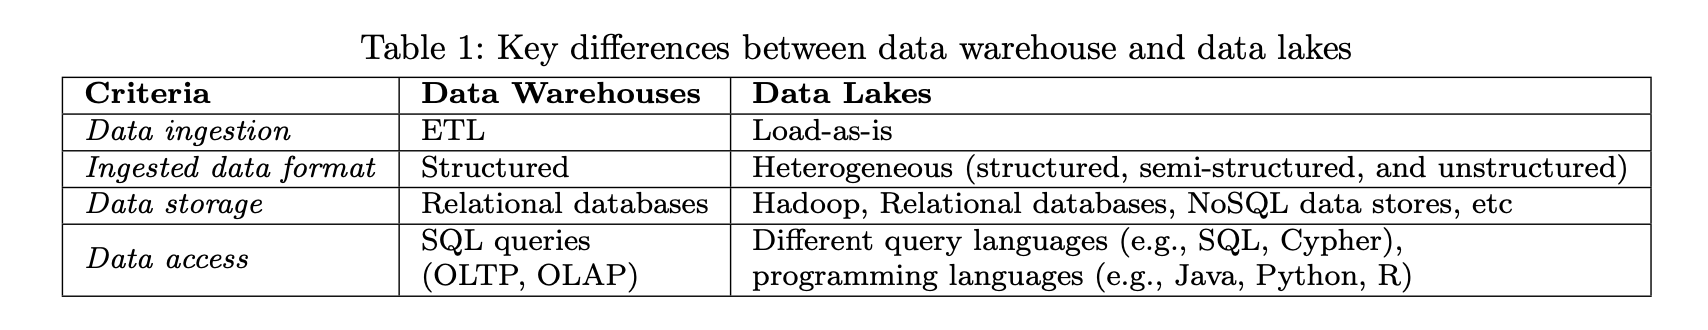
\includegraphics[scale=.4]{dw_data_lake}
\end{frame}


\begin{frame}{Data Warehouse vs. Data Lakes}
	\emph{A data warehouse (DW) manages, integrates, and aggregates data from multiple sources, and provides data analytics for decision making via multi-dimensional data cubes in data marts.} \vspace{.25cm}

\emph{In data warehouses, heterogeneous source datasets need to first go through the Extract/transform/load (ETL) process}\vspace{.25cm}

\emph{DW data is stored and handled as structured data in relational databases or cube structures.}\vspace{.25cm}
\end{frame}


\begin{frame}{Data Warehouse vs. Data Lakes}
	\emph{In data lakes the transformation step is delayed and data is loaded in its original structure (i.e., load-as-is) to reduce upfront cleaning and integration effort and to make full source data available for later data analysis (i.e., pay-as-you-go).} \vspace{.25cm}
	
	\emph{Data lakes aim to process more heterogeneous sources including semi-structured and unstructured sources, and to manage these different data models efficiently using multiple dedicated kinds of storage}\vspace{.25cm}
	
	\emph{DW usually applies (multi-dimensional extensions of) SQL queries, while a data lake may need to support different query languages (e.g., SQL, Cypher11, JSONiq12), and programming languages (e.g., Python, Java, R)}\vspace{.25cm}
\end{frame}


\begin{frame}{Data lakes and dataspaces}
	\emph{The early dataspace prototypes tackled the problems of how to organize, integrate, discover, and query the data from several loosely interrelated data sources. } \vspace{.25cm}
	
	\emph{ The dataspace concept can be considered a complement to the data lake approach supporting sovereign inter-organizational cooperation.}\vspace{.25cm}
\end{frame}
 \section{Use cases of data lakes}
 
 \begin{frame}{Multiple heterogeneous raw data inputs}
 	\emph{Alice is a scientist who studies the milling process, and she has two problems with the data.
 		\vspace{.25cm}
 		
 		First, vast and heterogeneous data is generated, which she needs to store and organize. Such production data includes binary image files from cameras, CSV and JSON files from different sensors, and ontologies enriched with her own annotation for the milling process. She hopes to store the heterogeneous data in raw formats, as transformation would be time-consuming, and might lose certain information and jeopardize her future research.
 		\vspace{.25cm}
 		
 		Second, instead of browsing through massive, diverse data files, she hopes to have a data management system, which provides her easy access to the raw data. A data lake would be a good solution to solve Alice’s problems.}
 \end{frame}

\begin{frame}{Use Case:}
	\begin{center}
		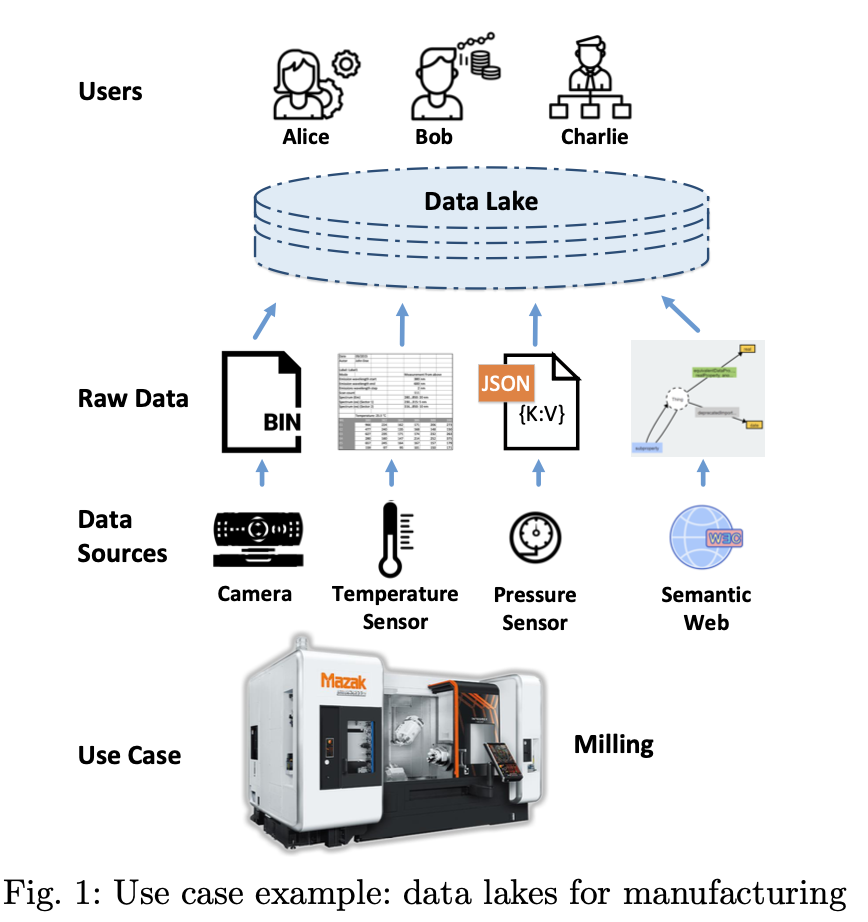
\includegraphics[scale=0.45]{data_lake_use_case.png}
	\end{center}

\end{frame}
 \begin{frame}{Data integration and transformation}
	\emph{ Bob is an industrial consultant, who has similar production data but in different formats, structures, and terminologies from Alice. Charlie is also a milling scientist but with a different research goal. He has another set of milling machines, sensors, and engineering models. For data analysis, he uses machine learning (ML) and runs Python scripts instead of merely queries. \vspace{.25cm}
		
	
		
		Both Bob and Charlie want to integrate and compare their data and results with Alice. The three users hope to have a data lake, which can combine these independent data sources, help them easily find the datasets relevant for their own use cases, transform the data flexibly, and provide query answering and data analytics.}
\end{frame}


 \begin{frame}{On-demand data processing and querying}
	\emph{  As a researcher, Alice has her research questions and solutions evolving with time. She may introduce a new sensor, which has different machine-generated data formats compared to the existing datasets in the data lake. She may have new queries or want to use the raw data in a different manner. \vspace{.25cm}
		
		In addition, in the beginning the usage of some raw datasets was unclear, which she just stored without using. Now she has created an engineering model for the unused data. Similar dynamic analytical requirements also apply to the use cases of Bob and Charlie. Therefore, they would like to have a data lake, which supports data processing, integration, and querying in an on-the-fly manner rather than being fixed from the beginning.}
\end{frame}

\section{DL Architecture}
\begin{frame}{DL Architecture}
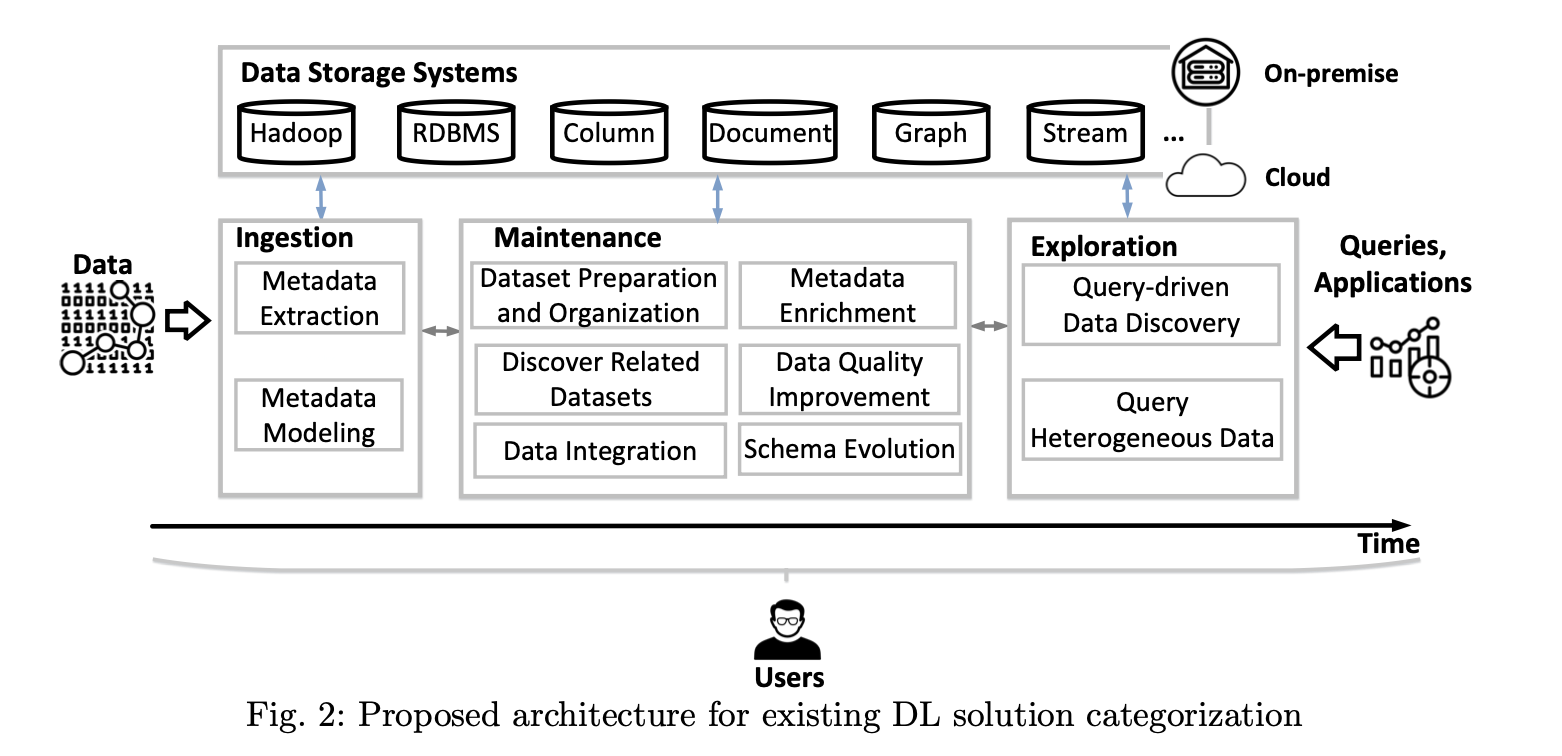
\includegraphics[scale=0.45]{archi}
\end{frame}

\begin{frame}
	Review this article : \emph{P. Sawadogo and J. Darmont. On data lake architectures and metadata management. Journal of Intelligent Information Systems, pages 1–24, 2020.}
\end{frame}
\end{document}